\documentclass[12pt, a4paper, simple]{eskdtext}

\usepackage{hyperref}
\usepackage{_env/gpi_global.env}
\usepackage{_env/gpi_report.env}
\usepackage{_sty/gpi_lst}
\usepackage{_sty/gpi_toc}
\usepackage{_sty/gpi_t}
\usepackage{_sty/gpi_p}
\usepackage{_sty/gpi_u}

% Код
% \ESKDletter{О}{Л}{Р}
% \def \gpiDocTypeNum {81}
% \def \gpiDocVer {00}
% \def \gpiCode {\ESKDtheLetterI\ESKDtheLetterII\ESKDtheLetterIII.\gpiStudentGroupName\gpiStudentGroupNum.\gpiStudentCard-0\gpiDocNum~\gpiDocTypeNum~\gpiDocVer}

\def \gpiDocTopic {Отчёт лабораторной работы №\gpiDocNum}

% Графа 1 (наименование изделия/документа)
% \ESKDcolumnI {\ESKDfontII \gpiTopic \\ \gpiDocTopic}

% Графа 2 (обозначение документа)
% \ESKDsignature {\gpiCode}

% Графа 9 (наименование или различительный индекс предприятия) задает команда
% \ESKDcolumnIX {\gpiDepartment}

% Графа 11 (фамилии лиц, подписывающих документ) задают команды
% \ESKDcolumnXIfI {\gpiStudentSurname}
% \ESKDcolumnXIfII {\gpiTeacherSurname}
% \ESKDcolumnXIfV {\gpiTeacherSurname}

\begin{document}
    \begin{ESKDtitlePage}
    \ESKDstyle{empty}
    \begin{center}
        \gpiMinEdu \\
        \gpiEdu \\
        \gpiKaf \\
    \end{center}

    \vfill

    \begin{center}
        \gpiTopic
    \end{center}

    \vfill

    \begin{center}
        \textbf{\gpiDocTopic} \\
        ПО ДИСЦИПЛИНЕ \gpiDiscipline \\
    \end{center}

    \vfill

    \begin{flushright}
        \begin{minipage}[t]{7cm}
            Выполнил:\\
            \PageTitleStudentInfo
            \PageTitleDateField
            \hspace{0pt}

            Проверил:\\
            \PageTitleTeacherInfo
            \PageTitleDateField
        \end{minipage}
    \end{flushright}

    \vfill

    \begin{center}
        \PageTitleCity~\ESKDtheYear
    \end{center}
\end{ESKDtitlePage}

    \ESKDstyle{empty}
    \begin{center}
        \textbf{\gpiDocTopic}
    \end{center}

    % = = = = = = = =
    \paragraph{} \textbf{Тема}: <<\gpiTopicRep>>

    \paragraph{} \textbf{Цель}:
    приобрести практические навыки разработки многооконных приложений на JavaFX для работы с базами данных.

    \paragraph{} \textbf{Что нужно сделать}:
    долго писать.
    Реализуй табличку с CRUD операциями.

    \paragraph{} \textbf{Разработка дизайна}:

    \begin{itemize}
        \item Главное меню (см. рис.~\ref{fig:View-Main}).
        \item Таблица справочника "Номенклатура" (см. рис.~\ref{fig:View-Table-Producer}).
        \item Форма справочника "Номенклатура" (см. рис.~\ref{fig:View-Form-Producer}).
        \item Таблица справочника "Единицы измерения".
        \item Форма справочника "Единицы измерения".
        \item Таблица справочника "Номенклатура".
        \item Форма справочника "Номенклатура".
        \item Таблица справочника "Клиенты".
        \item Форма справочника "Клиенты".
        \item Таблица документа "Сборка компьютера".
        \item Форма документа "Сборка компьютера".
    \end{itemize}

    \begin{figure}[!ph]
        \centering
        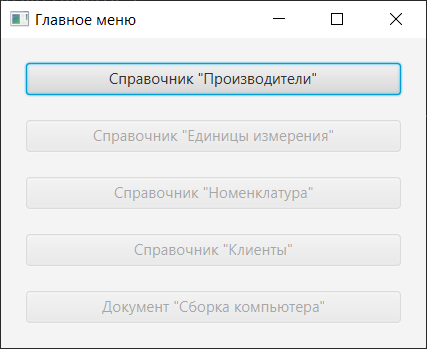
\includegraphics[]
            {_assets/View-Main.png}
        \caption{Главное меню}
        \label{fig:View-Main}
    \end{figure}

    \begin{figure}[!ph]
        \centering
        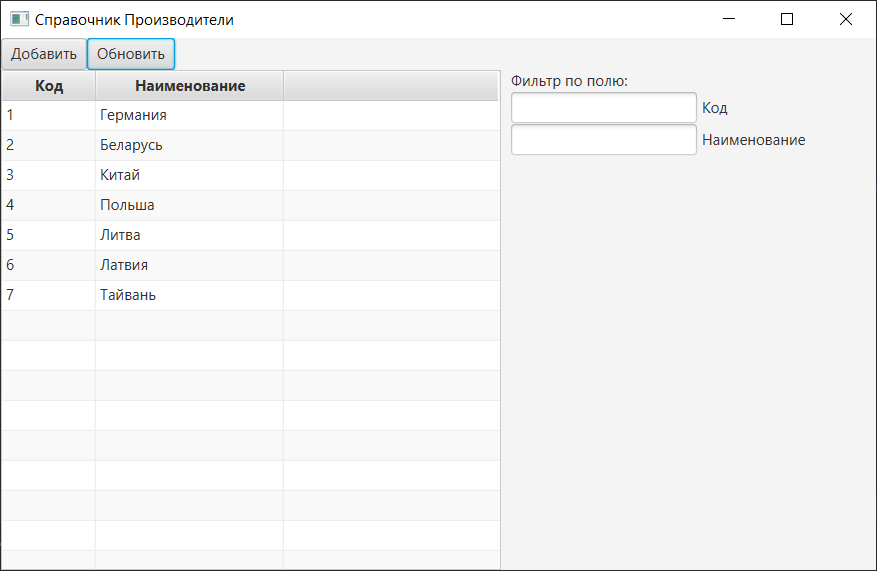
\includegraphics[width=16cm]
            {_assets/View-Table-Producer.png}
        \caption{Таблица справочника "Номенклатура"}
        \label{fig:View-Table-Producer}
    \end{figure}

    \begin{figure}[!ph]
        \centering
        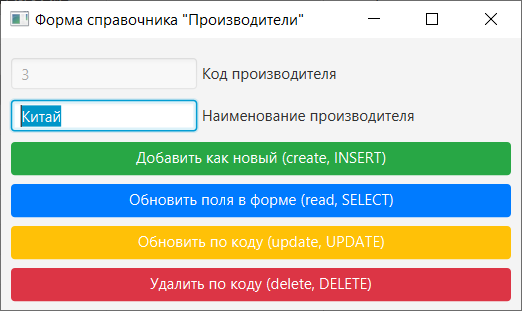
\includegraphics[]
            {_assets/View-Form-Producer.png}
        \caption{Форма справочника "Номенклатура"}
        \label{fig:View-Form-Producer}
    \end{figure}

    \newpage
    \paragraph{} \textbf{Исходный код}: 

    \begin{itemize}
        \item \textbf{Main.java} - главный класс программы
        \item \textbf{MainJavaFX.java} - главный класс графического интерфейса
        \item \textbf{Database.java} - класс, для работы с базой данных
    \end{itemize}

    \paragraph{} \textbf{Model - модели}:

    \begin{itemize}
        \item \textbf{ModelProducer.java} - модель справочника "Производители"
        \item \textbf{ModelUnitMeasure.java} - модель справочника "Единицы измерения"
        \item \textbf{ModelNomenclature.java} - модель справочника "Номенклатура"
        \item \textbf{ModelClients.java} - модель справочника "Клиенты"
        \item \textbf{ModelAssemblyComputer.java} - модель документа "Сборка компьютера"
    \end{itemize}

    \paragraph{} \textbf{Controller - контролеры}:

    \begin{itemize}
        \item \textbf{ControllerMain.java} - контроллер главного меню
        \item \textbf{ControllerTableProducer.java} - контроллер таблицы справочника "Производители"
        \item \textbf{ControllerTableUnitMeasure.java} - контроллер таблицы справочника "Единицы измерения"
        \item \textbf{ControllerTableNomenclature.java} - контроллер таблицы справочника "Номенклатура"
        \item \textbf{ControllerTableClients.java} - контроллер таблицы справочника "Клиенты"
        \item \textbf{ControllerTableAssemblyComputer.java} - контроллер таблицы документа "Сборка компьютера"
        \item[] \hspace{0pt}
        \item \textbf{ControllerFormProducer.java} - контроллер формы справочника "Производители"
        \item \textbf{ControllerFormUnitMeasure.java} - контроллер формы справочника "Единицы измерения"
        \item \textbf{ControllerFormNomenclature.java} - контроллер формы справочника "Номенклатура"
        \item \textbf{ControllerFormClients.java} - контроллер формы справочника "Клиенты"
        \item \textbf{ControllerFormAssemblyComputer.java} - контроллер формы справочника "Сборка компьютера"
    \end{itemize}

    \paragraph{} \textbf{View - дизайн}:

    \begin{itemize}
        \item \textbf{View-Main.fxml} - дизайн главного меню
        \item \textbf{View-Table-Producer.fxml} - дизайн таблицы справочника "Производители"
        \item \textbf{View-Table-Unit-measure.fxml} - дизайн таблицы справочника "Единицы измерения"
        \item \textbf{View-Table-Nomenclature.fxml} - дизайн таблицы справочника "Номенклатура"
        \item \textbf{View-Table-Clients.fxml} - дизайн таблицы справочника "Клиенты"
        \item \textbf{View-Table-Assembly-computer.fxml} - дизайн таблицы документа "Сборка компьютера"
        \item[] \hspace{0pt}
        \item \textbf{View-Form-Producer.fxml} - дизайн формы справочника "Производители"
        \item \textbf{View-Form-Unit-measure.fxml} - дизайн формы справочника "Единицы измерения"
        \item \textbf{View-Form-Nomenclature.fxml} - дизайн формы справочника "Номенклатура"
        \item \textbf{View-Form-Clients.fxml} - дизайн формы справочника "Клиенты"
        \item \textbf{View-Form-Assembly-computer.fxml} - дизайн формы документа "Сборка компьютера"
    \end{itemize}

    \lstinputlisting[language=java, name=src/main/java/com/example/../Main.java]
    {../sources/src/main/java/com/example/spp_2sem_po4_galanin_lab4/Main.java}

    \lstinputlisting[language=java, name=src/main/java/com/example/../MainJavaFX.java]
    {../sources/src/main/java/com/example/spp_2sem_po4_galanin_lab4/MainJavaFX.java}


    \lstinputlisting[language=java, name=src/main/java/com/example/../Database.java]
    {../sources/src/main/java/com/example/spp_2sem_po4_galanin_lab4/Database.java}


    \lstinputlisting[language=xml, name=src/main/resources/com/example/../View-Main.fxml]
    {../sources/src/main/resources/com/example/spp_2sem_po4_galanin_lab4/View-Main.fxml}

    \lstinputlisting[language=java, name=src/main/java/com/example/../ControllerMain.java]
    {../sources/src/main/java/com/example/spp_2sem_po4_galanin_lab4/ControllerMain.java}


   
    \lstinputlisting[language=xml, name=src/main/resources/com/example/../View-Table-Producer.fxml]
    {../sources/src/main/resources/com/example/spp_2sem_po4_galanin_lab4/View-Table-Producer.fxml}

    \lstinputlisting[language=java, name=src/main/java/com/example/../ControllerTableProducer.java]
    {../sources/src/main/java/com/example/spp_2sem_po4_galanin_lab4/ControllerTableProducer.java}


    \lstinputlisting[language=xml, name=src/main/resources/com/example/../View-Form-Producer.fxml]
    {../sources/src/main/resources/com/example/spp_2sem_po4_galanin_lab4/View-Form-Producer.fxml}

    \lstinputlisting[language=java, name=src/main/java/com/example/../ControllerFormProducer.java]
    {../sources/src/main/java/com/example/spp_2sem_po4_galanin_lab4/ControllerFormProducer.java}

%     \begin{lstlisting}[caption=Вывод в консоль]
%  Hello, World!
% \end{lstlisting}

    \paragraph{} \textbf{Вывод}:
    Реализовали операции CRUD: create, read, update, delete.

    Создали TableView, который выводит содержание таблицы.

    Создали форму,
    которая по нажатию кнопки "(create, INSERT)",
    создаст новый кортедж в таблице;
    которая по нажатию кнопки "(read, SELECT)",
    обновит поля в форме;
    которая по нажатию кнопки "(update, UPDATE)",
    обновит кортедж в базе данных;
    которая по нажатию кнопки "(delete, DELETE)",
    удалит кортедж в базе данных.

    При выборе поля из TableView, реализовали открытие формы.

    % = = = = = = = =
    \newpage
    % \addcontentsline{toc}{section}{Список использованных источников}
    % \section*{Список использованных источников}
    \paragraph{} \textbf{Список использованных источников}:
    \begin{enumerate}
        \item[1.] IntelliJ database connection error: java.sql.SQLException: No suitable driver found. SOLVED - YouTube [Электронный ресурс]
        - Режим доступа: \url{https://www.youtube.com/watch?v=lks1NZCnvL8}.
        Дата~доступа:~02.05.2022.
        \item[2.] Releases · xerial/sqlite-jdbc [Электронный ресурс]
        - Режим доступа: \url{https://github.com/xerial/sqlite-jdbc/releases}.
        Дата~доступа:~02.05.2022.
        \item[3.] JDBC CRUD Example Tutorial [Электронный ресурс]
        - Режим доступа: \url{https://www.javaguides.net/2018/10/jdbc-crud-example-tutorial.html}.
        Дата~доступа:~03.05.2022.
        \item[4.] java - Проверить наличие таблицы в БД и если она не существует создать. JDBC - Stack Overflow на русском [Электронный ресурс]
        - Режим доступа: \url{https://ru.stackoverflow.com/questions/623653/%D0%9F%D1%80%D0%BE%D0%B2%D0%B5%D1%80%D0%B8%D1%82%D1%8C-%D0%BD%D0%B0%D0%BB%D0%B8%D1%87%D0%B8%D0%B5-%D1%82%D0%B0%D0%B1%D0%BB%D0%B8%D1%86%D1%8B-%D0%B2-%D0%91%D0%94-%D0%B8-%D0%B5%D1%81%D0%BB%D0%B8-%D0%BE%D0%BD%D0%B0-%D0%BD%D0%B5-%D1%81%D1%83%D1%89%D0%B5%D1%81%D1%82%D0%B2%D1%83%D0%B5%D1%82-%D1%81%D0%BE%D0%B7%D0%B4%D0%B0%D1%82%D1%8C-jdbc}.
        Дата~доступа:~03.05.2022.
        \item[5.] SQL INSERT INTO Statement [Электронный ресурс]
        - Режим доступа: \url{https://www.w3schools.com/sql/sql_insert.asp}.
        Дата~доступа:~03.05.2022.
        \item[6.] SQL SELECT Statement [Электронный ресурс]
        - Режим доступа: \url{https://www.w3schools.com/sql/sql_select.asp}.
        Дата~доступа:~03.05.2022.
        \item[7.] SQL UPDATE Statement [Электронный ресурс]
        - Режим доступа: \url{https://www.w3schools.com/sql/sql_update.asp}.
        Дата~доступа:~03.05.2022.
        \item[8.] SQL DELETE Statement [Электронный ресурс]
        - Режим доступа: \url{https://www.w3schools.com/sql/sql_delete.asp}.
        Дата~доступа:~03.05.2022.
        \item[9.] SQL DROP TABLE Statement [Электронный ресурс]
        - Режим доступа: \url{https://www.w3schools.com/sql/sql_drop_table.asp}.
        Дата~доступа:~03.05.2022.
        \item[10.] Как создать исполняемый jar файл в IntelliJ IDEA - YouTube [Электронный ресурс]
        - Режим доступа: \url{https://www.youtube.com/watch?v=tA8rEz_xFrQ}.
        Дата~доступа:~01.05.2022.
        \item[11.] Export JavaFX 11, 15 or 17 projects into an executable jar file with IntelliJ [2022] - YouTube [Электронный ресурс]
        - Режим доступа: \url{https://www.youtube.com/watch?v=F8ahBtXkQzU}.
        Дата~доступа:~01.05.2022.
        \item[12.] JavaFX Tutorial for Beginners - CRUD Application Part 1 - YouTube [Электронный ресурс]
        - Режим доступа: \url{https://www.youtube.com/watch?v=CGWRwpeihE8}.
        Дата~доступа:~19.05.2022.
        \item[13.] JavaFX Tutorial for Beginners - CRUD Application  with JavaFX and MySQL Part 2 - YouTube [Электронный ресурс]
        - Режим доступа: \url{https://www.youtube.com/watch?v=kpnnXit2br0}.
        Дата~доступа:~20.05.2022.
        \item[14.] DemoCRUD-JavaFX/MainController.java at master · xemacscode/DemoCRUD-JavaFX [Электронный ресурс]
        - Режим доступа: \url{https://github.com/xemacscode/DemoCRUD-JavaFX/blob/master/src/org/xemacscode/demo/MainController.java}.
        Дата~доступа:~20.05.2022.
        \item[15.] Passing Parameters JavaFX FXML - Stack Overflow [Электронный ресурс]
        - Режим доступа: \url{https://stackoverflow.com/questions/14187963/passing-parameters-javafx-fxml#answer-14190310}.
        Дата~доступа:~27.05.2022.
    \end{enumerate}
    \newpage
\end{document}
